\documentclass[a4paper,11pt]{article}

% Kodovani (cestiny) v dokumentu: utf-8
%\usepackage[cp1250]{inputenc}	% Omezena stredoevropska kodova stranka, pouze MSW.
\usepackage[utf8]{inputenc}	% Doporucujeme pouzivat UTF-8 (unicode).

\usepackage[margin=2cm]{geometry}
\newtoks\jmenopraktika \newtoks\jmeno \newtoks\datum
\newtoks\obor \newtoks\skupina \newtoks\rocnik \newtoks\semestr
\newtoks\cisloulohy \newtoks\jmenoulohy
\newtoks\tlak \newtoks\teplota \newtoks\vlhkost

\jmenopraktika={Fyzikální praktikum 3}
\jmeno={Lukáš Lejdar}
\datum={15. dubna 2025}
\obor={F}
\skupina={Út 14:00}

\cisloulohy={1}
\jmenoulohy={Pohyb nábojů v elektrickém a magnetickém poli}

%%%%%%%%%%% Uzitecne balicky:
\usepackage[czech]{babel}

\usepackage{graphicx}
\usepackage{amsmath}
\usepackage{xspace}
\usepackage{url}
\usepackage{indentfirst}
\usepackage{wrapfig}
\usepackage{xcolor}
\usepackage{subfig}
\usepackage{subcaption}
\usepackage{enumitem}
\usepackage{tikzsymbols}
\usepackage{newfloat}
\usepackage{float}

\DeclareFloatingEnvironment[fileext=lof]{graph}
\captionsetup[graph]{labelformat=simple, labelsep=colon, name=Graf}

%%%%%% Zamezeni parchantu:
\widowpenalty 10000 \clubpenalty 10000 \displaywidowpenalty 10000
%%%%%% Parametry pro moznost vsazeni vetsiho poctu obrazku na stranku
\setcounter{topnumber}{3}	  % max. pocet floatu nahore (specifikace t)
\setcounter{bottomnumber}{3}	  % max. pocet floatu dole (specifikace b)
\setcounter{totalnumber}{6}	  % max. pocet floatu na strance celkem
\renewcommand\topfraction{0.9}	  % max podil stranky pro floaty nahore
\renewcommand\bottomfraction{0.9} % max podil stranky pro floaty dole
\renewcommand\textfraction{0.1}	  % min podil stranky, ktery musi obsahovat text
\intextsep=8mm \textfloatsep=8mm  %\intextsep pro ulozeni [h] floatu a \textfloatsep pro [b] or [t]

% Tecky za cisly sekci:
\renewcommand{\thesection}{\arabic{section}.}
\renewcommand{\thesubsection}{\thesection\arabic{subsection}.}
% Jednopismenna mezera mezi cislem a nazvem kapitoly:
\makeatletter \def\@seccntformat#1{\csname the#1\endcsname\hspace{1ex}} \makeatother
%
\newcommand{\vsn}[4]{\ensuremath{#1 =} #2(#3)\,#4}
\newcommand{\vrn}[6]{\ensuremath{#1 =} (#2 $\pm$ #3)\,#4 ($p=$ #5\,\%, $\nu=$ #6)}

\newcommand*\circled[1]{\tikz[baseline=(char.base)]{
		\node[shape=circle,draw,inner sep=1pt] (char) {#1};}}

%%%%%%%%%%%%%%%%%%%%%%%%%%%%%%%%%%%%%%%%%%%%%%%%%%%%%%%%%%%%%%%%%%%%%%%%%%%%%%%
% Zacatek dokumentu
%%%%%%%%%%%%%%%%%%%%%%%%%%%%%%%%%%%%%%%%%%%%%%%%%%%%%%%%%%%%%%%%%%%%%%%%%%%%%%%

\begin{document}

\thispagestyle{empty}

{
\begin{center}
\sf 
{\Large Ústav fyziky a technologií plazmatu Přírodovědecké fakulty Masarykovy univerzity} \\
\bigskip
{\huge \bfseries FYZIKÁLNÍ PRAKTIKUM} \\
\bigskip
{\Large \the\jmenopraktika}
\end{center}

\bigskip

\sf
\noindent
\setlength{\arrayrulewidth}{1pt}
\begin{tabular*}{\textwidth}{@{\extracolsep{\fill}} l l}
\large {\bfseries Zpracoval:}  \the\jmeno & \large  {\bfseries Naměřeno:} \the\datum\\[2mm]
\large  {\bfseries Obor:} \the\obor  \hspace{40mm}  {\bfseries Skupina:} \the\skupina %
&\large {\bfseries Testováno:}\\
\\
\hline
\end{tabular*}
}

\bigskip

{
\sf
\noindent \begin{tabular}{p{4cm} p{0.6\textwidth}}
\Large  Úloha č. {\bfseries \the\cisloulohy:} \par
\smallskip
&\Large \bfseries \the\jmenoulohy  \\[2mm]
\end{tabular}
}

\vskip1cm

\section{Úvod}

Toto praktikum je zaměřené na způsoby, jakými se dá usměrňovat, nebo zaostřovat svazek elektronů, pomocí cívek a elektrod.
Na těchto principech fungovali například první televize, která bude i předmětem měření. 
 
\section{Teorie}

Schéma uspořádání součástí televize je vidět na obrázku 1. Z katody vzadu televize vyletují elektrony, které jsou potom urychlené napětím na anodách. Svazek je potom možné fokusovat, nebo vychylovat a jeho stopu uvidíme na luminiscenčním stínítku televize. 

\begin{figure}[h]
    \centering
    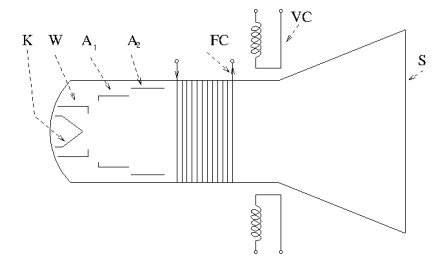
\includegraphics[width=0.5\textwidth]{obrazovka.jpg}
    \caption{ Schématické znázornění uspořádání obrazovky s magnetickou fokusací a s magnetickým
vychylováním. K - katoda, W - Wehneltův válec, $ A_1 $  a $ A_2 $  - anody, F C - fokusační cívka, V C -
dva páry vychylovacích cívek, S - stínítko. }
\end{figure}

Zaostření elektronů můžeme provádět krátkou magentickou čočkou. Je to krátká cívka, jejíž rotační magnetické pole fokusuje původně divergentní svazek do bodové stopy na stínítku. Pro její ohniskovou vzdálenost platí vztah

\begin{equation}
f = 98 \frac{r}{n^2} \frac{U_a}{ I_f^2},
\end{equation}

\noindent
kde $ r $  je poloměr cívky, $ n $ počet závitů, $ I_f $ proud tekoucí cívkou a $ U_a $ anodové napětí.

Pokud je vychylovací cívka vypnutá, bude svazek dopadat doprostřed obrazovky. Pro jeho výchylku $ y $ od středu při zvyšování magnetického pole jde odvodit druhý vztah

\begin{equation}
y = \sqrt{\frac{e}{2m}} L_1 L_2 \frac{B}{\sqrt{U_a} },
\end{equation}

\noindent
kde $ L_1 $ je délka působení vychylovacích cívek, $ L_2 $ je vzdálenost ke stínítku a B je indukované magnetické pole, které je zároveň přímo úměrné vychylovacímu proudu $ I_v $ . 

\section{Postup měření}

Schéma pro praktické měření pohybu nábojů je na obrázku (2). Anodové napětí a fokusační a vychylovací proudy se dají ovládat pomocí připojených potenciometrů a všechny tyto veličiny se měří zapojením dvou ampérmetrů a voltmetru. 

\begin{figure}[h]
    \centering
    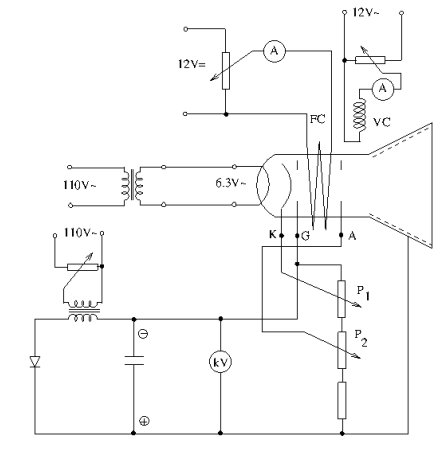
\includegraphics[width=0.6\textwidth]{schema.jpg}
    \caption{Elektrické schéma zapojení obvodů pro měření na obrazovce}
\end{figure}

\newpage

\section{Výsledky měření}

\subsection{Ohnisková vzdálenost}

Obrazovku jsem zapojil podle schematu na obrázku 1 a zkontroloval, že funguje zaostřování i vychylování posunováním jezdců potenciometrů. Pro ověření vztahu (1) jsem začal na nízkém anodovém napětí $ U_a $ a potom měnil fokusační proud, tak aby byl obraz ostrý. Do grafu 1 jsem potom vykreslil lineární závislost (1) a z fitu přímkou určil ohniskovou vzdálenost

\begin{equation}
f = 45.2 \pm 0.2 \text{ cm}
\end{equation}

\begin{table}[h]
    \begin{minipage}{.40\linewidth}
        \centering
        \begin{tabular}{| c c |}
            \hline
            $ U_a $ (kV)  &  $ I_f $ (mA) \\
            \hline
            2.00 & 93.5 \\
            1.95 & 91.9 \\
            1.90 & 91.5 \\
            1.85 & 90.4 \\
            1.80 & 88.1 \\
            1.75 & 87.0 \\
            1.70 & 86.1 \\
            1.65 & 84.2 \\
            1.60 & 82.2 \\
            1.55 & 81.3 \\
            1.50 & 79.5 \\
            \hline
        \end{tabular}
        \caption{Naměřené napětí a fokusační proudy při ostrém obrazu na stínítku}
    \end{minipage} 
    \hfill
    \begin{minipage}{.5\linewidth}
        \centering
        \resizebox{\textwidth}{!}{ % GNUPLOT: LaTeX picture with Postscript
\begingroup
  \makeatletter
  \providecommand\color[2][]{%
    \GenericError{(gnuplot) \space\space\space\@spaces}{%
      Package color not loaded in conjunction with
      terminal option `colourtext'%
    }{See the gnuplot documentation for explanation.%
    }{Either use 'blacktext' in gnuplot or load the package
      color.sty in LaTeX.}%
    \renewcommand\color[2][]{}%
  }%
  \providecommand\includegraphics[2][]{%
    \GenericError{(gnuplot) \space\space\space\@spaces}{%
      Package graphicx or graphics not loaded%
    }{See the gnuplot documentation for explanation.%
    }{The gnuplot epslatex terminal needs graphicx.sty or graphics.sty.}%
    \renewcommand\includegraphics[2][]{}%
  }%
  \providecommand\rotatebox[2]{#2}%
  \@ifundefined{ifGPcolor}{%
    \newif\ifGPcolor
    \GPcolorfalse
  }{}%
  \@ifundefined{ifGPblacktext}{%
    \newif\ifGPblacktext
    \GPblacktexttrue
  }{}%
  % define a \g@addto@macro without @ in the name:
  \let\gplgaddtomacro\g@addto@macro
  % define empty templates for all commands taking text:
  \gdef\gplbacktext{}%
  \gdef\gplfronttext{}%
  \makeatother
  \ifGPblacktext
    % no textcolor at all
    \def\colorrgb#1{}%
    \def\colorgray#1{}%
  \else
    % gray or color?
    \ifGPcolor
      \def\colorrgb#1{\color[rgb]{#1}}%
      \def\colorgray#1{\color[gray]{#1}}%
      \expandafter\def\csname LTw\endcsname{\color{white}}%
      \expandafter\def\csname LTb\endcsname{\color{black}}%
      \expandafter\def\csname LTa\endcsname{\color{black}}%
      \expandafter\def\csname LT0\endcsname{\color[rgb]{1,0,0}}%
      \expandafter\def\csname LT1\endcsname{\color[rgb]{0,1,0}}%
      \expandafter\def\csname LT2\endcsname{\color[rgb]{0,0,1}}%
      \expandafter\def\csname LT3\endcsname{\color[rgb]{1,0,1}}%
      \expandafter\def\csname LT4\endcsname{\color[rgb]{0,1,1}}%
      \expandafter\def\csname LT5\endcsname{\color[rgb]{1,1,0}}%
      \expandafter\def\csname LT6\endcsname{\color[rgb]{0,0,0}}%
      \expandafter\def\csname LT7\endcsname{\color[rgb]{1,0.3,0}}%
      \expandafter\def\csname LT8\endcsname{\color[rgb]{0.5,0.5,0.5}}%
    \else
      % gray
      \def\colorrgb#1{\color{black}}%
      \def\colorgray#1{\color[gray]{#1}}%
      \expandafter\def\csname LTw\endcsname{\color{white}}%
      \expandafter\def\csname LTb\endcsname{\color{black}}%
      \expandafter\def\csname LTa\endcsname{\color{black}}%
      \expandafter\def\csname LT0\endcsname{\color{black}}%
      \expandafter\def\csname LT1\endcsname{\color{black}}%
      \expandafter\def\csname LT2\endcsname{\color{black}}%
      \expandafter\def\csname LT3\endcsname{\color{black}}%
      \expandafter\def\csname LT4\endcsname{\color{black}}%
      \expandafter\def\csname LT5\endcsname{\color{black}}%
      \expandafter\def\csname LT6\endcsname{\color{black}}%
      \expandafter\def\csname LT7\endcsname{\color{black}}%
      \expandafter\def\csname LT8\endcsname{\color{black}}%
    \fi
  \fi
    \setlength{\unitlength}{0.0500bp}%
    \ifx\gptboxheight\undefined%
      \newlength{\gptboxheight}%
      \newlength{\gptboxwidth}%
      \newsavebox{\gptboxtext}%
    \fi%
    \setlength{\fboxrule}{0.5pt}%
    \setlength{\fboxsep}{1pt}%
    \definecolor{tbcol}{rgb}{1,1,1}%
\begin{picture}(5328.00,3600.00)%
    \gplgaddtomacro\gplbacktext{%
      \csname LTb\endcsname%%
      \put(726,440){\makebox(0,0)[r]{\strut{}$1400$}}%
      \put(726,860){\makebox(0,0)[r]{\strut{}$1500$}}%
      \put(726,1280){\makebox(0,0)[r]{\strut{}$1600$}}%
      \put(726,1700){\makebox(0,0)[r]{\strut{}$1700$}}%
      \put(726,2119){\makebox(0,0)[r]{\strut{}$1800$}}%
      \put(726,2539){\makebox(0,0)[r]{\strut{}$1900$}}%
      \put(726,2959){\makebox(0,0)[r]{\strut{}$2000$}}%
      \put(726,3379){\makebox(0,0)[r]{\strut{}$2100$}}%
      \put(858,220){\makebox(0,0){\strut{}$0.006$}}%
      \put(1537,220){\makebox(0,0){\strut{}$0.0065$}}%
      \put(2216,220){\makebox(0,0){\strut{}$0.007$}}%
      \put(2895,220){\makebox(0,0){\strut{}$0.0075$}}%
      \put(3573,220){\makebox(0,0){\strut{}$0.008$}}%
      \put(4252,220){\makebox(0,0){\strut{}$0.0085$}}%
      \put(4931,220){\makebox(0,0){\strut{}$0.009$}}%
    }%
    \gplgaddtomacro\gplfronttext{%
      \csname LTb\endcsname%%
      \put(99,1909){\rotatebox{-270}{\makebox(0,0){\strut{}}}}%
      \put(2894,-66){\makebox(0,0){\strut{}}}%
      \csname LTb\endcsname%%
      \put(3944,3206){\makebox(0,0)[r]{\strut{}fit}}%
    }%
    \gplbacktext
    \put(0,0){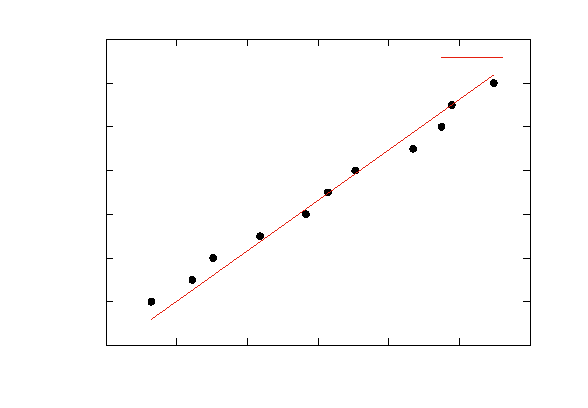
\includegraphics[width={266.40bp},height={180.00bp}]{ohnisko}}%
    \gplfronttext
  \end{picture}%
\endgroup
 }
        \captionsetup{type=graph}
        \caption{Závislost čtverce fokusačního proudu na anodovém napětí}
    \end{minipage} 
\end{table}

\subsection{Vychýlení svazku}

Druhým úkolem bylo ověřit platnost vztahu (2). Podle něj by měla výchylka svazku $ y $ být přímo úměrná magnetické indukci $ y \propto B \propto I_v $ a taky $ y \propto U_a^{-0.5} $. Není ale úplně jednoduché zjistit, kde přesně je střed obrazovky, od kterého by se mělo $ y $  měřit. Namísto toho použiju střídavý proud $ I_v $ , což na stínítku vytvoří čáru a výchylka $ y $ je polovina délky této čáry. Budu měřit výchylky jednou při konstantním napětí a podruhé při konstantním proudu a zjistím, jestli je y na veličinách přímo úměrné jednotlivě. Naměřená data jsou v tabulkách 2 a závislosti jsou vykreslené do grafů 2 a 3. 

\begin{table}[h]
    \begin{minipage}[b]{.48\linewidth}
        \centering
        \resizebox{\textwidth}{!}{ % GNUPLOT: LaTeX picture with Postscript
\begingroup
  \makeatletter
  \providecommand\color[2][]{%
    \GenericError{(gnuplot) \space\space\space\@spaces}{%
      Package color not loaded in conjunction with
      terminal option `colourtext'%
    }{See the gnuplot documentation for explanation.%
    }{Either use 'blacktext' in gnuplot or load the package
      color.sty in LaTeX.}%
    \renewcommand\color[2][]{}%
  }%
  \providecommand\includegraphics[2][]{%
    \GenericError{(gnuplot) \space\space\space\@spaces}{%
      Package graphicx or graphics not loaded%
    }{See the gnuplot documentation for explanation.%
    }{The gnuplot epslatex terminal needs graphicx.sty or graphics.sty.}%
    \renewcommand\includegraphics[2][]{}%
  }%
  \providecommand\rotatebox[2]{#2}%
  \@ifundefined{ifGPcolor}{%
    \newif\ifGPcolor
    \GPcolorfalse
  }{}%
  \@ifundefined{ifGPblacktext}{%
    \newif\ifGPblacktext
    \GPblacktexttrue
  }{}%
  % define a \g@addto@macro without @ in the name:
  \let\gplgaddtomacro\g@addto@macro
  % define empty templates for all commands taking text:
  \gdef\gplbacktext{}%
  \gdef\gplfronttext{}%
  \makeatother
  \ifGPblacktext
    % no textcolor at all
    \def\colorrgb#1{}%
    \def\colorgray#1{}%
  \else
    % gray or color?
    \ifGPcolor
      \def\colorrgb#1{\color[rgb]{#1}}%
      \def\colorgray#1{\color[gray]{#1}}%
      \expandafter\def\csname LTw\endcsname{\color{white}}%
      \expandafter\def\csname LTb\endcsname{\color{black}}%
      \expandafter\def\csname LTa\endcsname{\color{black}}%
      \expandafter\def\csname LT0\endcsname{\color[rgb]{1,0,0}}%
      \expandafter\def\csname LT1\endcsname{\color[rgb]{0,1,0}}%
      \expandafter\def\csname LT2\endcsname{\color[rgb]{0,0,1}}%
      \expandafter\def\csname LT3\endcsname{\color[rgb]{1,0,1}}%
      \expandafter\def\csname LT4\endcsname{\color[rgb]{0,1,1}}%
      \expandafter\def\csname LT5\endcsname{\color[rgb]{1,1,0}}%
      \expandafter\def\csname LT6\endcsname{\color[rgb]{0,0,0}}%
      \expandafter\def\csname LT7\endcsname{\color[rgb]{1,0.3,0}}%
      \expandafter\def\csname LT8\endcsname{\color[rgb]{0.5,0.5,0.5}}%
    \else
      % gray
      \def\colorrgb#1{\color{black}}%
      \def\colorgray#1{\color[gray]{#1}}%
      \expandafter\def\csname LTw\endcsname{\color{white}}%
      \expandafter\def\csname LTb\endcsname{\color{black}}%
      \expandafter\def\csname LTa\endcsname{\color{black}}%
      \expandafter\def\csname LT0\endcsname{\color{black}}%
      \expandafter\def\csname LT1\endcsname{\color{black}}%
      \expandafter\def\csname LT2\endcsname{\color{black}}%
      \expandafter\def\csname LT3\endcsname{\color{black}}%
      \expandafter\def\csname LT4\endcsname{\color{black}}%
      \expandafter\def\csname LT5\endcsname{\color{black}}%
      \expandafter\def\csname LT6\endcsname{\color{black}}%
      \expandafter\def\csname LT7\endcsname{\color{black}}%
      \expandafter\def\csname LT8\endcsname{\color{black}}%
    \fi
  \fi
    \setlength{\unitlength}{0.0500bp}%
    \ifx\gptboxheight\undefined%
      \newlength{\gptboxheight}%
      \newlength{\gptboxwidth}%
      \newsavebox{\gptboxtext}%
    \fi%
    \setlength{\fboxrule}{0.5pt}%
    \setlength{\fboxsep}{1pt}%
    \definecolor{tbcol}{rgb}{1,1,1}%
\begin{picture}(5328.00,3600.00)%
    \gplgaddtomacro\gplbacktext{%
      \csname LTb\endcsname%%
      \put(682,704){\makebox(0,0)[r]{\strut{}$2$}}%
      \put(682,972){\makebox(0,0)[r]{\strut{}$3$}}%
      \put(682,1239){\makebox(0,0)[r]{\strut{}$4$}}%
      \put(682,1507){\makebox(0,0)[r]{\strut{}$5$}}%
      \put(682,1774){\makebox(0,0)[r]{\strut{}$6$}}%
      \put(682,2042){\makebox(0,0)[r]{\strut{}$7$}}%
      \put(682,2309){\makebox(0,0)[r]{\strut{}$8$}}%
      \put(682,2577){\makebox(0,0)[r]{\strut{}$9$}}%
      \put(682,2844){\makebox(0,0)[r]{\strut{}$10$}}%
      \put(682,3112){\makebox(0,0)[r]{\strut{}$11$}}%
      \put(682,3379){\makebox(0,0)[r]{\strut{}$12$}}%
      \put(814,484){\makebox(0,0){\strut{}$20$}}%
      \put(1271,484){\makebox(0,0){\strut{}$30$}}%
      \put(1729,484){\makebox(0,0){\strut{}$40$}}%
      \put(2186,484){\makebox(0,0){\strut{}$50$}}%
      \put(2644,484){\makebox(0,0){\strut{}$60$}}%
      \put(3101,484){\makebox(0,0){\strut{}$70$}}%
      \put(3559,484){\makebox(0,0){\strut{}$80$}}%
      \put(4016,484){\makebox(0,0){\strut{}$90$}}%
      \put(4474,484){\makebox(0,0){\strut{}$100$}}%
      \put(4931,484){\makebox(0,0){\strut{}$110$}}%
    }%
    \gplgaddtomacro\gplfronttext{%
      \csname LTb\endcsname%%
      \put(209,2041){\rotatebox{-270}{\makebox(0,0){\strut{}$ y $ (cm)}}}%
      \put(2872,154){\makebox(0,0){\strut{}$ I_v (mA) $}}%
      \csname LTb\endcsname%%
      \put(2510,3021){\makebox(0,0)[r]{\strut{}fit $ U_a = 1750 $ V}}%
      \csname LTb\endcsname%%
      \put(2510,2801){\makebox(0,0)[r]{\strut{}fit $ U_a = 2000 $ V}}%
    }%
    \gplbacktext
    \put(0,0){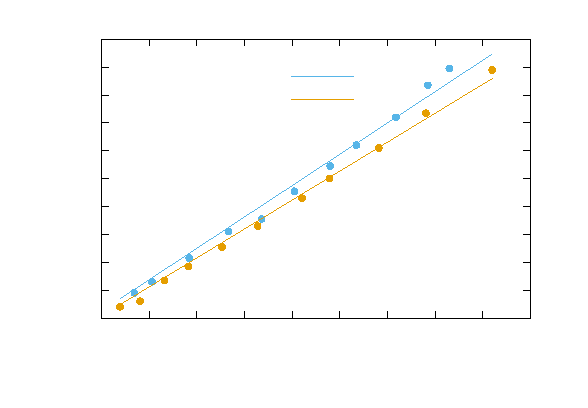
\includegraphics[width={266.40bp},height={180.00bp}]{vychylovani_Ifkonst}}%
    \gplfronttext
  \end{picture}%
\endgroup
 }
        \captionsetup{type=graph}
        \caption{Závislost výchylky $ y $ na vychylovacím proudu $ I_v $  }
    \end{minipage} 
    \hfill
    \begin{minipage}[b]{.48\linewidth}
        \centering
        \resizebox{\textwidth}{!}{ % GNUPLOT: LaTeX picture with Postscript
\begingroup
  \makeatletter
  \providecommand\color[2][]{%
    \GenericError{(gnuplot) \space\space\space\@spaces}{%
      Package color not loaded in conjunction with
      terminal option `colourtext'%
    }{See the gnuplot documentation for explanation.%
    }{Either use 'blacktext' in gnuplot or load the package
      color.sty in LaTeX.}%
    \renewcommand\color[2][]{}%
  }%
  \providecommand\includegraphics[2][]{%
    \GenericError{(gnuplot) \space\space\space\@spaces}{%
      Package graphicx or graphics not loaded%
    }{See the gnuplot documentation for explanation.%
    }{The gnuplot epslatex terminal needs graphicx.sty or graphics.sty.}%
    \renewcommand\includegraphics[2][]{}%
  }%
  \providecommand\rotatebox[2]{#2}%
  \@ifundefined{ifGPcolor}{%
    \newif\ifGPcolor
    \GPcolorfalse
  }{}%
  \@ifundefined{ifGPblacktext}{%
    \newif\ifGPblacktext
    \GPblacktexttrue
  }{}%
  % define a \g@addto@macro without @ in the name:
  \let\gplgaddtomacro\g@addto@macro
  % define empty templates for all commands taking text:
  \gdef\gplbacktext{}%
  \gdef\gplfronttext{}%
  \makeatother
  \ifGPblacktext
    % no textcolor at all
    \def\colorrgb#1{}%
    \def\colorgray#1{}%
  \else
    % gray or color?
    \ifGPcolor
      \def\colorrgb#1{\color[rgb]{#1}}%
      \def\colorgray#1{\color[gray]{#1}}%
      \expandafter\def\csname LTw\endcsname{\color{white}}%
      \expandafter\def\csname LTb\endcsname{\color{black}}%
      \expandafter\def\csname LTa\endcsname{\color{black}}%
      \expandafter\def\csname LT0\endcsname{\color[rgb]{1,0,0}}%
      \expandafter\def\csname LT1\endcsname{\color[rgb]{0,1,0}}%
      \expandafter\def\csname LT2\endcsname{\color[rgb]{0,0,1}}%
      \expandafter\def\csname LT3\endcsname{\color[rgb]{1,0,1}}%
      \expandafter\def\csname LT4\endcsname{\color[rgb]{0,1,1}}%
      \expandafter\def\csname LT5\endcsname{\color[rgb]{1,1,0}}%
      \expandafter\def\csname LT6\endcsname{\color[rgb]{0,0,0}}%
      \expandafter\def\csname LT7\endcsname{\color[rgb]{1,0.3,0}}%
      \expandafter\def\csname LT8\endcsname{\color[rgb]{0.5,0.5,0.5}}%
    \else
      % gray
      \def\colorrgb#1{\color{black}}%
      \def\colorgray#1{\color[gray]{#1}}%
      \expandafter\def\csname LTw\endcsname{\color{white}}%
      \expandafter\def\csname LTb\endcsname{\color{black}}%
      \expandafter\def\csname LTa\endcsname{\color{black}}%
      \expandafter\def\csname LT0\endcsname{\color{black}}%
      \expandafter\def\csname LT1\endcsname{\color{black}}%
      \expandafter\def\csname LT2\endcsname{\color{black}}%
      \expandafter\def\csname LT3\endcsname{\color{black}}%
      \expandafter\def\csname LT4\endcsname{\color{black}}%
      \expandafter\def\csname LT5\endcsname{\color{black}}%
      \expandafter\def\csname LT6\endcsname{\color{black}}%
      \expandafter\def\csname LT7\endcsname{\color{black}}%
      \expandafter\def\csname LT8\endcsname{\color{black}}%
    \fi
  \fi
    \setlength{\unitlength}{0.0500bp}%
    \ifx\gptboxheight\undefined%
      \newlength{\gptboxheight}%
      \newlength{\gptboxwidth}%
      \newsavebox{\gptboxtext}%
    \fi%
    \setlength{\fboxrule}{0.5pt}%
    \setlength{\fboxsep}{1pt}%
    \definecolor{tbcol}{rgb}{1,1,1}%
\begin{picture}(5328.00,3600.00)%
    \gplgaddtomacro\gplbacktext{%
      \csname LTb\endcsname%%
      \put(682,704){\makebox(0,0)[r]{\strut{}$6$}}%
      \put(682,1239){\makebox(0,0)[r]{\strut{}$7$}}%
      \put(682,1774){\makebox(0,0)[r]{\strut{}$8$}}%
      \put(682,2309){\makebox(0,0)[r]{\strut{}$9$}}%
      \put(682,2844){\makebox(0,0)[r]{\strut{}$10$}}%
      \put(682,3379){\makebox(0,0)[r]{\strut{}$11$}}%
      \put(814,484){\makebox(0,0){\strut{}$2.2$}}%
      \put(1329,484){\makebox(0,0){\strut{}$2.25$}}%
      \put(1843,484){\makebox(0,0){\strut{}$2.3$}}%
      \put(2358,484){\makebox(0,0){\strut{}$2.35$}}%
      \put(2872,484){\makebox(0,0){\strut{}$2.4$}}%
      \put(3387,484){\makebox(0,0){\strut{}$2.45$}}%
      \put(3902,484){\makebox(0,0){\strut{}$2.5$}}%
      \put(4416,484){\makebox(0,0){\strut{}$2.55$}}%
      \put(4931,484){\makebox(0,0){\strut{}$2.6$}}%
    }%
    \gplgaddtomacro\gplfronttext{%
      \csname LTb\endcsname%%
      \put(209,2041){\rotatebox{-270}{\makebox(0,0){\strut{}$ y $ (cm)}}}%
      \put(2872,154){\makebox(0,0){\strut{} $ U_a^{-1/2} \cdot 10^{-2} $  $ (kV^{-1/2})  $ }}%
      \csname LTb\endcsname%%
      \put(2608,3165){\makebox(0,0)[r]{\strut{}fit $ I_v = 82.0  $ mA}}%
      \csname LTb\endcsname%%
      \put(2608,2945){\makebox(0,0)[r]{\strut{}fit $I_v = 62.8$ mA}}%
    }%
    \gplbacktext
    \put(0,0){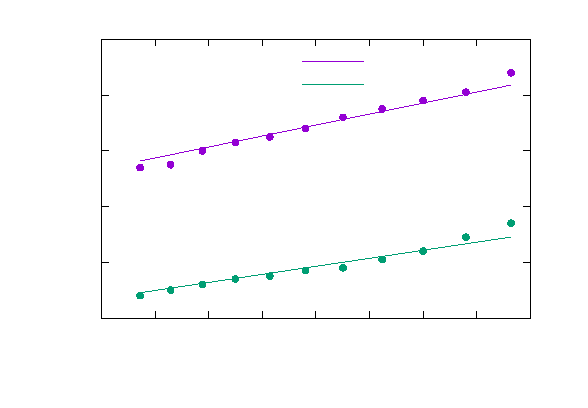
\includegraphics[width={266.40bp},height={180.00bp}]{vychylovani_Ivkonst}}%
    \gplfronttext
  \end{picture}%
\endgroup
 }
        \captionsetup{type=graph}
        \caption{Závislost výchylky $ y $ na urychlovacím napětí $ U_a $ }
    \end{minipage} 
\end{table}

\newpage

\begin{figure}[h]
    \footnotesize
    \centering
    \subfloat[$ I_v \approx 82 $ mA ]{
    \begin{tabular}{| c c c c |}
        \hline
        $ U_a $ (V) & $ I_f $ (mA) & $ I_v $ (mA) & $ 2 y $ (cm)   \\
        \hline
        1500 & 75.8 & 83.8 & 20.8 \\
        1550 & 80.3 & 83.5 & 20.1 \\
        1600 & 81.0 & 82.0 & 19.8 \\
        1650 & 82.4 & 81.3 & 19.5 \\
        1700 & 85.7 & 81.3 & 19.2 \\
        1750 & 86.1 & 82.4 & 18.8 \\
        1800 & 88.7 & 82.8 & 18.5 \\
        1850 & 88.2 & 83.0 & 18.3 \\
        1900 & 88.1 & 81.2 & 18.0 \\
        1950 & 91.8 & 81.6 & 17.5 \\ 
        2000 & 93.9 & 82.3 & 17.4 \\
        \hline
    \end{tabular}
    }
    \hspace{1cm}
    \subfloat[$ I_v \approx 62.8 $  mA ]{
    \begin{tabular}{| c c c c |}
        \hline
        $ U_a $ (V) & $ I_f $ (mA) & $ I_v $ (mA) & $ 2 y $ (cm)   \\
        \hline
        1500 & 79.4 & 62.7 & 15.4 \\
        1550 & 81.6 & 62.8 & 14.9 \\
        1600 & 83.9 & 62.9 & 14.4 \\
        1650 & 83.6 & 62.2 & 14.1 \\
        1700 & 86.9 & 62.8 & 13.8 \\
        1750 & 88.2 & 62.7 & 13.7 \\
        1800 & 88.7 & 62.9 & 13.5 \\
        1850 & 89.1 & 62.8 & 13.4 \\
        1900 & 91.5 & 62.7 & 13.2 \\
        1950 & 91.3 & 62.8 & 13.0 \\
        2000 & 94.3 & 63.0 & 12.8 \\
        \hline
    \end{tabular}
    }
    \vspace{1cm}
    \subfloat[$ U_a \approx 1750 $ V ]{
    \begin{tabular}{| c c c c |}
        \hline
        $ U_a $ (V) & $ I_f $ (mA) & $ I_v $ (mA) & $ 2 y $ (cm)   \\
        \hline
        1750 & 83.1 & 93.0 & 21.9 \\
        1750 & 84.1 & 88.5 & 20.7 \\
        1750 & 85.7 & 81.8 & 18.4 \\
        1750 & 86.3 & 73.5 & 16.4 \\
        1750 & 86.3 & 68.0 & 14.9 \\
        1750 & 86.3 & 60.5 & 13.1 \\ 
        1750 & 86.3 & 53.6 & 11.1 \\
        1750 & 86.3 & 46.7 & 10.2 \\
        1750 & 86.3 & 38.4 & 8.30 \\
        1750 & 86.3 & 30.6 & 6.60 \\
        1750 & 86.3 & 26.9 & 5.80 \\
        \hline
    \end{tabular}
    }
    \hspace{1cm}
    \subfloat[$ U_a \approx 2000 $ V]{ 
    \begin{tabular}{| c c c c |}
        \hline
        $ U_a $ (V) & $ I_f $ (mA) & $ I_v $ (mA) & $ 2 y $ (cm)   \\
        \hline
        2000 & 92.2 & 102 & 21.8 \\
        2000 & 92.2 & 88.1 & 18.7 \\
        2000 & 92.2 & 78.2 & 16.2 \\
        2000 & 92.2 & 67.9 & 14.0 \\
        2000 & 92.2 & 62.1 & 12.6 \\
        2000 & 92.2 & 52.8 & 10.6 \\
        2000 & 92.2 & 45.3 & 9.10 \\
        2000 & 92.2 & 38.2 & 7.70 \\
        2000 & 92.2 & 33.2 & 6.70 \\
        2000 & 92.2 & 28.1 & 5.20 \\
        2000 & 92.2 & 23.9 & 4.80 \\
        \hline
    \end{tabular}
    }
    \captionsetup{type=table}
    \caption{Naměřená data vychýlení bodu na obrazovce v závislosti na urychlovacím napětí $ U_a $ a vychylovacím proudu $ I_v $.  }
\end{figure}

\begin{figure}[H]
    \centering
    \resizebox{0.7\textwidth}{!}{ % GNUPLOT: LaTeX picture with Postscript
\begingroup
  \makeatletter
  \providecommand\color[2][]{%
    \GenericError{(gnuplot) \space\space\space\@spaces}{%
      Package color not loaded in conjunction with
      terminal option `colourtext'%
    }{See the gnuplot documentation for explanation.%
    }{Either use 'blacktext' in gnuplot or load the package
      color.sty in LaTeX.}%
    \renewcommand\color[2][]{}%
  }%
  \providecommand\includegraphics[2][]{%
    \GenericError{(gnuplot) \space\space\space\@spaces}{%
      Package graphicx or graphics not loaded%
    }{See the gnuplot documentation for explanation.%
    }{The gnuplot epslatex terminal needs graphicx.sty or graphics.sty.}%
    \renewcommand\includegraphics[2][]{}%
  }%
  \providecommand\rotatebox[2]{#2}%
  \@ifundefined{ifGPcolor}{%
    \newif\ifGPcolor
    \GPcolorfalse
  }{}%
  \@ifundefined{ifGPblacktext}{%
    \newif\ifGPblacktext
    \GPblacktexttrue
  }{}%
  % define a \g@addto@macro without @ in the name:
  \let\gplgaddtomacro\g@addto@macro
  % define empty templates for all commands taking text:
  \gdef\gplbacktext{}%
  \gdef\gplfronttext{}%
  \makeatother
  \ifGPblacktext
    % no textcolor at all
    \def\colorrgb#1{}%
    \def\colorgray#1{}%
  \else
    % gray or color?
    \ifGPcolor
      \def\colorrgb#1{\color[rgb]{#1}}%
      \def\colorgray#1{\color[gray]{#1}}%
      \expandafter\def\csname LTw\endcsname{\color{white}}%
      \expandafter\def\csname LTb\endcsname{\color{black}}%
      \expandafter\def\csname LTa\endcsname{\color{black}}%
      \expandafter\def\csname LT0\endcsname{\color[rgb]{1,0,0}}%
      \expandafter\def\csname LT1\endcsname{\color[rgb]{0,1,0}}%
      \expandafter\def\csname LT2\endcsname{\color[rgb]{0,0,1}}%
      \expandafter\def\csname LT3\endcsname{\color[rgb]{1,0,1}}%
      \expandafter\def\csname LT4\endcsname{\color[rgb]{0,1,1}}%
      \expandafter\def\csname LT5\endcsname{\color[rgb]{1,1,0}}%
      \expandafter\def\csname LT6\endcsname{\color[rgb]{0,0,0}}%
      \expandafter\def\csname LT7\endcsname{\color[rgb]{1,0.3,0}}%
      \expandafter\def\csname LT8\endcsname{\color[rgb]{0.5,0.5,0.5}}%
    \else
      % gray
      \def\colorrgb#1{\color{black}}%
      \def\colorgray#1{\color[gray]{#1}}%
      \expandafter\def\csname LTw\endcsname{\color{white}}%
      \expandafter\def\csname LTb\endcsname{\color{black}}%
      \expandafter\def\csname LTa\endcsname{\color{black}}%
      \expandafter\def\csname LT0\endcsname{\color{black}}%
      \expandafter\def\csname LT1\endcsname{\color{black}}%
      \expandafter\def\csname LT2\endcsname{\color{black}}%
      \expandafter\def\csname LT3\endcsname{\color{black}}%
      \expandafter\def\csname LT4\endcsname{\color{black}}%
      \expandafter\def\csname LT5\endcsname{\color{black}}%
      \expandafter\def\csname LT6\endcsname{\color{black}}%
      \expandafter\def\csname LT7\endcsname{\color{black}}%
      \expandafter\def\csname LT8\endcsname{\color{black}}%
    \fi
  \fi
    \setlength{\unitlength}{0.0500bp}%
    \ifx\gptboxheight\undefined%
      \newlength{\gptboxheight}%
      \newlength{\gptboxwidth}%
      \newsavebox{\gptboxtext}%
    \fi%
    \setlength{\fboxrule}{0.5pt}%
    \setlength{\fboxsep}{1pt}%
    \definecolor{tbcol}{rgb}{1,1,1}%
\begin{picture}(8640.00,7200.00)%
    \gplgaddtomacro\gplbacktext{%
      \csname LTb\endcsname%%
      \put(4687,795){\makebox(0,0){\strut{}$20$}}%
      \csname LTb\endcsname%%
      \put(4283,948){\makebox(0,0){\strut{}$30$}}%
      \csname LTb\endcsname%%
      \put(3878,1101){\makebox(0,0){\strut{}$40$}}%
      \csname LTb\endcsname%%
      \put(3473,1254){\makebox(0,0){\strut{}$50$}}%
      \csname LTb\endcsname%%
      \put(3068,1407){\makebox(0,0){\strut{}$60$}}%
      \csname LTb\endcsname%%
      \put(2663,1561){\makebox(0,0){\strut{}$70$}}%
      \csname LTb\endcsname%%
      \put(2258,1714){\makebox(0,0){\strut{}$80$}}%
      \csname LTb\endcsname%%
      \put(1854,1867){\makebox(0,0){\strut{}$90$}}%
      \csname LTb\endcsname%%
      \put(1449,2020){\makebox(0,0){\strut{}$100$}}%
      \csname LTb\endcsname%%
      \put(1044,2173){\makebox(0,0){\strut{}$110$}}%
      \csname LTb\endcsname%%
      \put(7755,2646){\makebox(0,0){\strut{}$2.2$}}%
      \csname LTb\endcsname%%
      \put(7412,2417){\makebox(0,0){\strut{}$2.25$}}%
      \csname LTb\endcsname%%
      \put(7068,2189){\makebox(0,0){\strut{}$2.3$}}%
      \csname LTb\endcsname%%
      \put(6725,1960){\makebox(0,0){\strut{}$2.35$}}%
      \csname LTb\endcsname%%
      \put(6382,1732){\makebox(0,0){\strut{}$2.4$}}%
      \csname LTb\endcsname%%
      \put(6039,1503){\makebox(0,0){\strut{}$2.45$}}%
      \csname LTb\endcsname%%
      \put(5695,1275){\makebox(0,0){\strut{}$2.5$}}%
      \csname LTb\endcsname%%
      \put(5352,1046){\makebox(0,0){\strut{}$2.55$}}%
      \csname LTb\endcsname%%
      \put(5009,817){\makebox(0,0){\strut{}$2.6$}}%
      \put(999,2263){\makebox(0,0)[r]{\strut{}$2$}}%
      \put(999,2596){\makebox(0,0)[r]{\strut{}$3$}}%
      \put(999,2930){\makebox(0,0)[r]{\strut{}$4$}}%
      \put(999,3263){\makebox(0,0)[r]{\strut{}$5$}}%
      \put(999,3596){\makebox(0,0)[r]{\strut{}$6$}}%
      \put(999,3929){\makebox(0,0)[r]{\strut{}$7$}}%
      \put(999,4262){\makebox(0,0)[r]{\strut{}$8$}}%
      \put(999,4594){\makebox(0,0)[r]{\strut{}$9$}}%
      \put(999,4927){\makebox(0,0)[r]{\strut{}$10$}}%
      \put(999,5260){\makebox(0,0)[r]{\strut{}$11$}}%
      \put(999,5593){\makebox(0,0)[r]{\strut{}$12$}}%
      \put(999,5926){\makebox(0,0)[r]{\strut{}$13$}}%
    }%
    \gplgaddtomacro\gplfronttext{%
      \csname LTb\endcsname%%
      \put(7395,6307){\makebox(0,0)[r]{\strut{}$ I_v = 82.0 $ mA}}%
      \csname LTb\endcsname%%
      \put(7395,6087){\makebox(0,0)[r]{\strut{}$ I_v = 62.8 $ mA}}%
      \csname LTb\endcsname%%
      \put(7395,5867){\makebox(0,0)[r]{\strut{}$ U_a = 1750 $ V}}%
      \csname LTb\endcsname%%
      \put(7395,5647){\makebox(0,0)[r]{\strut{}$ U_a = 2000 $ V}}%
      \csname LTb\endcsname%%
      \put(2558,1315){\makebox(0,0){\strut{}$ I_v $ (mA)}}%
      \put(7847,1604){\makebox(0,0){\strut{}$ U_a^{-1/2} \cdot 10^{-2} $  $ (kV^{-1/2})  $ }}%
      \put(201,4095){\makebox(0,0){\strut{}$ y $ (cm)}}%
    }%
    \gplbacktext
    \put(0,0){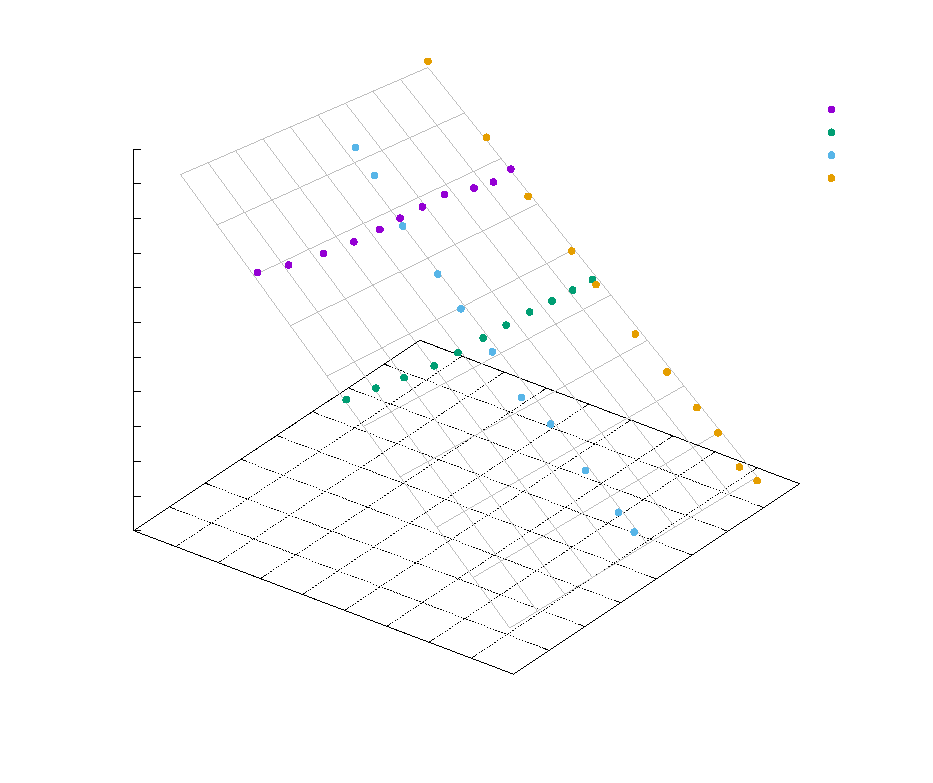
\includegraphics[width={432.00bp},height={360.00bp}]{3dvychylovani}}%
    \gplfronttext
  \end{picture}%
\endgroup
 }
    \captionsetup{type=graph}
    \caption{Závislost výchylky $ y $ na urychlovacím napětí $ U_a^{-\frac{1}{2}} $ a vychylovacím napětí $ I_v $.    }
\end{figure}

\newpage

\section{Závěr}

 V první části úlohy jsem ověřil vztah (1) pro ohniskovou vzdálenost magnetické čočky a určil její hodnotu $ f = 45.2 \pm 0.2 $ mm. Přes dobrou přesnost tato hodnota určitě není správná, protože televize je dlouhá jenom asi 30 cm. Myslím, že hodnoty všechny hodnoty byli změřené dostatečně přesně, takže závěrem je že vztah (1) alespoň v mé aparatuře není úplně přesný. Potvrdilo se ale, že mezi napětím $ U_a $ proudem $ I_f^2 $ a ohniskovou vzdáleností $ f $  existuje lineární vztah, jak ukazuje graf 1. 

 V druhé části jsem měl za úkol ověřit, že výchylka bodu na stínítku je přímo úměrná magnetickému poli, tedy i vychylovacímu proudu $ B \propto I_v $ a energii elektronů, nebo napětí $ E^{-0.5} \propto U_a^{-0.5} $. Obě tyto závislosti se potvrdili jak ukazují grafy 2, 3 a 4.

\begin{thebibliography}{0}
\bibitem{tabulky} návod k úloze ~\url{https://is.muni.cz/auth/el/sci/jaro2025/F4210/um/fp3-1_obrazovka.pdf}.   
\end{thebibliography}

\end{document}
